\documentclass[a4paper]{article}
\usepackage[english]{babel}
\usepackage[utf8]{inputenc}
\usepackage{amsmath}
\usepackage{graphicx}
\usepackage{natbib}
\usepackage{float}
\usepackage[margin=1.2in]{geometry}
\usepackage{caption}
\usepackage{subcaption}
\usepackage{url}
\usepackage{bm}
\usepackage{wasysym}
\usepackage{pdflscape}
\usepackage{tabularx}
\usepackage{hhline}
\usepackage{geometry}
\usepackage{longtable}
\usepackage{amsmath,bm}
\usepackage{array}
\usepackage[colorinlistoftodos]{todonotes}
\usepackage{siunitx}
\usepackage{mathtools}
\usepackage{comment}
\usepackage{setspace}
%\usepackage{hyperref}
\onehalfspacing

\mathchardef\mhyphen="2D

\newcommand{\pder}[2][]{\frac{\partial#1}{\partial#2}}
\newcommand{\pdder}[2][]{\frac{\partial^2#1}{\partial#2 ^2}}
\newcolumntype{P}[1]{>{\centering\arraybackslash}p{#1}}

\graphicspath{{./plots/}}

%----------------------------------------------------------------------------------------

\title{Time Series\\ Exercise 1}

\author{Rory Hetherington (200471193)}

\date{13 Feb 2017}

\begin{document}


\maketitle

%----------------------------------------------------------------------------------------

\section*{Question 1}
The provided code is ran in R. Summary statistics are generated (Table \ref{tab:summary_stats}) and the data is plotted (Figure \ref{fig:ex1q1_rplot}). It can be seen in Fig. \ref{fig:ex1q1_rplot} that there is seasonality in the data. 

Spikes occur every 10 years, where for every 4 spikes, there is one large one. Large spikes occur with a period of roughly 40 years.

\begin{longtable}{ p{.1\textwidth} P{.1\textwidth}  P{.1\textwidth}    P{.1\textwidth}    P{.1\textwidth}   P{.1\textwidth} }
	\hline \hline  \vspace{0.2cm}
	 \textbf{Min.}  & \textbf{1st Qu.}  &  \textbf{Median}  &  \textbf{Mean}   &  \textbf{3rd Qu.} &   \textbf{Max.}\\ 
	\hline 
	 39.0 &  348.2 & 771.0  &  1538.0   &  2567.0  &   6991.0     \\	
	\hline \hline
	\caption{Summary statistics for the annual number of lynx trapped at Mackenzie River between 1821 and 1934.}
	\label{tab:summary_stats}
\end{longtable}

\begin{figure}
	\centering
	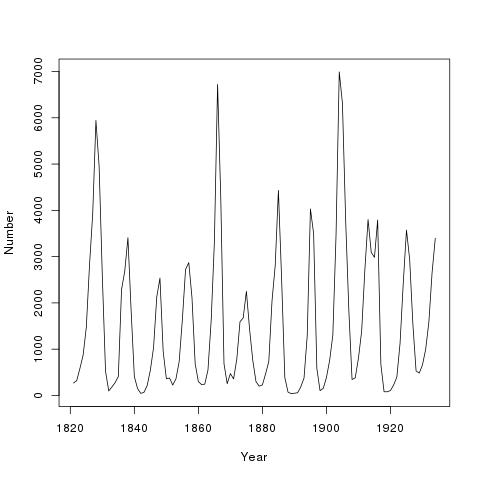
\includegraphics[width=0.6\textwidth]{ex1q1_rplot}
	\caption{Annual number of lynx trapped at Mackenzie River between 1821 and 1934.}
	\label{fig:ex1q1_rplot}
\end{figure}

\section*{Question 2}
In order to obtain a 95\% confidence interval, we use the following formulation

\begin{equation}
\hat{y} \pm 1.96 \sqrt{\sigma^2},
\end{equation}

here $\hat{y}$ is the approximated average and $\sigma^2$ the variance, both at time $t=2000$. To estimate $\hat{y}$, a linear model is fitted to obtain an estimation for the mean $\hat{y}$

\begin{equation}    \label{eq:yhat}
\hat{y}= \hat{\alpha}+\hat{\beta}t, \qquad \textrm{for} \quad t=2000.
\end{equation}

\begin{equation}    \label{eqs:alpha_beta}
\hat{\alpha} = \overline{X}- \hat{\beta} \overline{t}, \qquad
\hat{\beta} = \frac{\sum_{i=1}^{n}(X_i-\overline{X})(t_i-\overline{t})}{\sum_{i=1}^{n}(t_i-\overline{t})^2}.
\end{equation}   

From \eqref{eq:yhat} and \eqref{eqs:alpha_beta} we find $\hat{y}=34.1077$.



\end{document}